\section{Process and methodology}
\label{sec:process-approach}
	
	The main effort of the current stage of the project is to develop a formal ontology. This corresponds to Step \ref{step:5} of the process described in \cite[3--15]{d2.01-2017} and repeated in Section \ref{sec:context}.	
	
	This section expands and addresses in detail the process of defining and implementing an OWL eProcurement ontology. The underlying assumption is that the conceptual data model developed at Step \ref{step:3} serves as an input for the creation of the ontology, and that this process shall be automatic. 
	
	In addition to producing the ontology as an artefact, we also need to validates its fitness to represent existing data and test whether the functional and non-functional requirements are respected. Figure \ref{fig:process-overview} depicts the sequence of steps as a BPMN process diagram \cite{bpmn-introduction}. 
	
	\begin{figure}[!ht]		
		\centering
		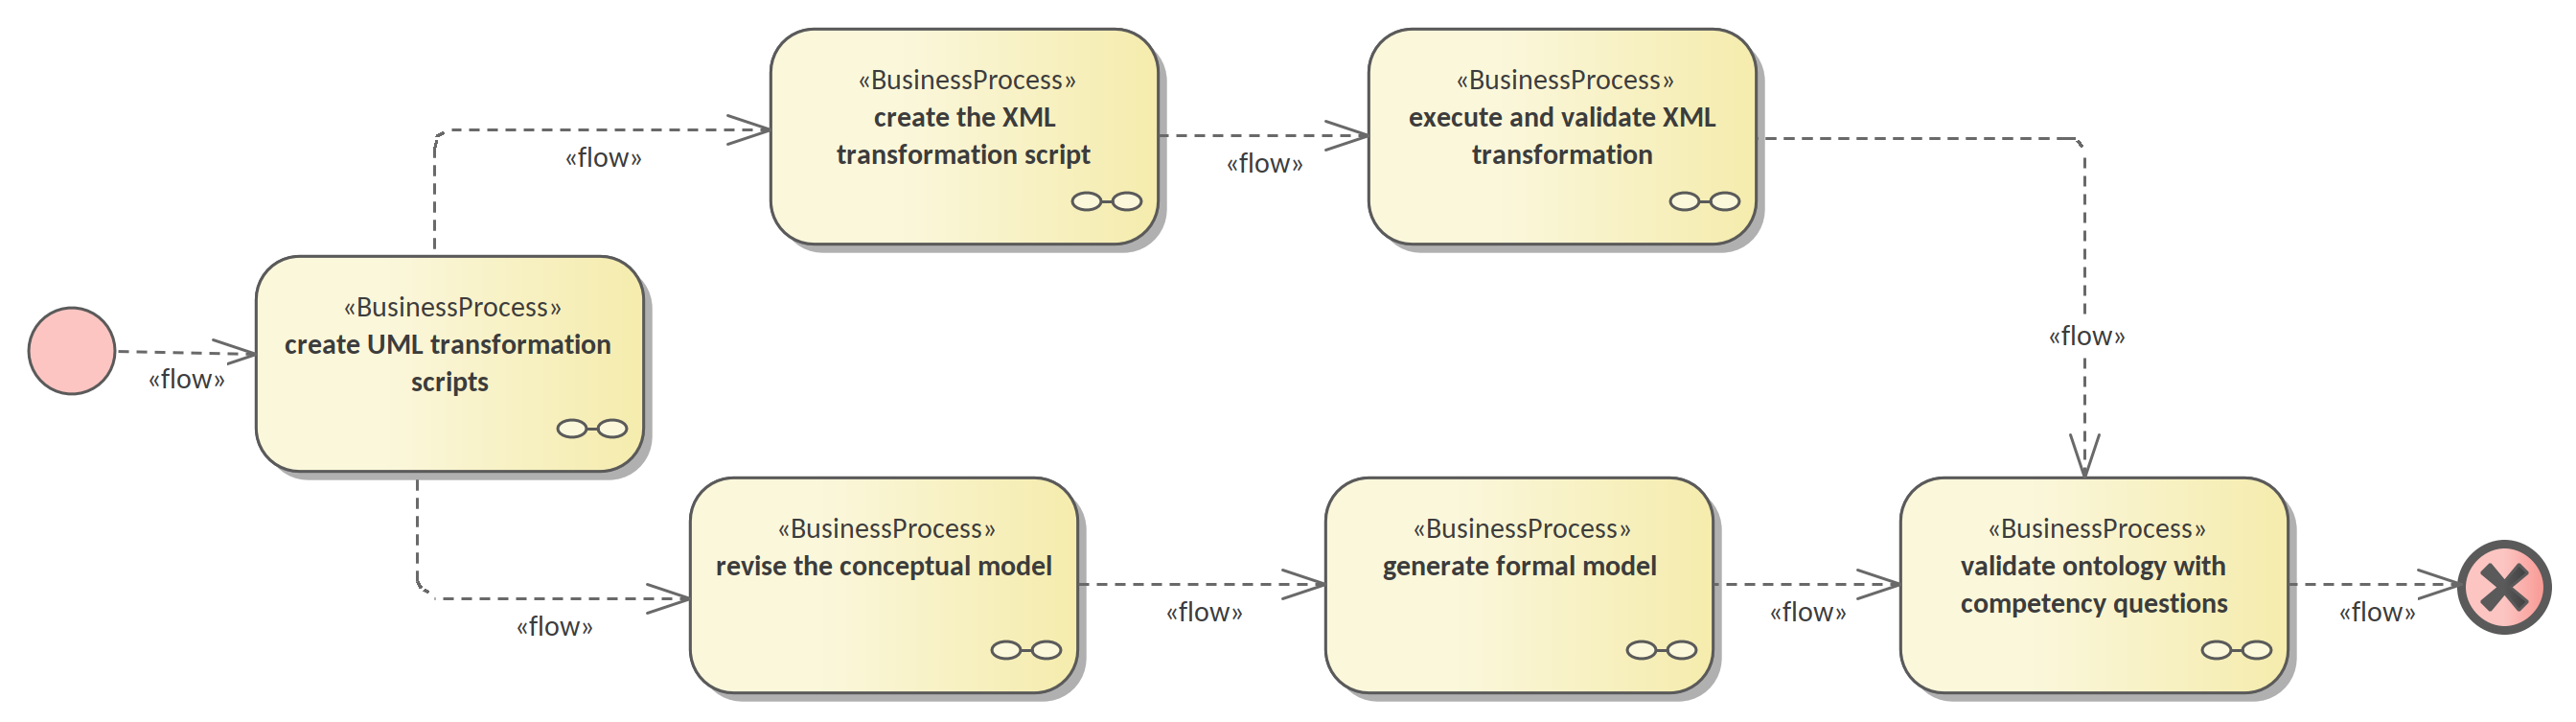
\includegraphics[width=\textwidth]{../img/processOverview.png}
		\caption{The main steps to implementing and validating the formal eProcurement ontology}
		\label{fig:process-overview}
	\end{figure}

	The conceptual model serves as the single source of truth, the process starts with development of a series of transformations scripts. The conceptual model needs to be adjusted in order to fit a set of UML modelling conventions \citep{costetchi2020b} making it suitable input for the transformation scripts. Provided that the conceptual model  conforms, the transformation can be executed. Finally, the validation of the formal ontology can be performed using the existing eProcurement data.
	
	
	%	after the creation of the UML transformation scripts, which also sets in place the ontology architecture, this document, and the UML conventions \citep{costetchi2020b}
	The existing eProcurement data needs to be transformed from XML into RDF format. So, in parallel, after the UML transformations are created and along with them, the ontology architecture and UML conventions, then a set of XML transformation scripts can be developed. Once they are ready, they need to be executed on previously selected datasets, to convert them into RDF data instantiating the formal ontology. Only then, when the datasets are available, the ontology can be validated. 
	
	The next subsections describe each of these six steps in more detail in order to provide rationale and introduce each artefact in part.
	
	\subsection{UML transformation scripts generation}
	\label{sec:uml-transformation}
	
	The process starts with authoring two documents laying the foundations of the entire process: the ontology architecture and the UML modelling conventions \citep{costetchi2020b}. The main purpose of the ontology architecture (this document) specifications is to describe why the ontology is being built, what its intended uses are, who the end-users are, and which requirements the ontology should fulfil. Moreover, it states how the ontology should be structured in order to facilitate maintenance and usage patterns.
	
	
	\begin{figure}[!ht]		
		\centering
		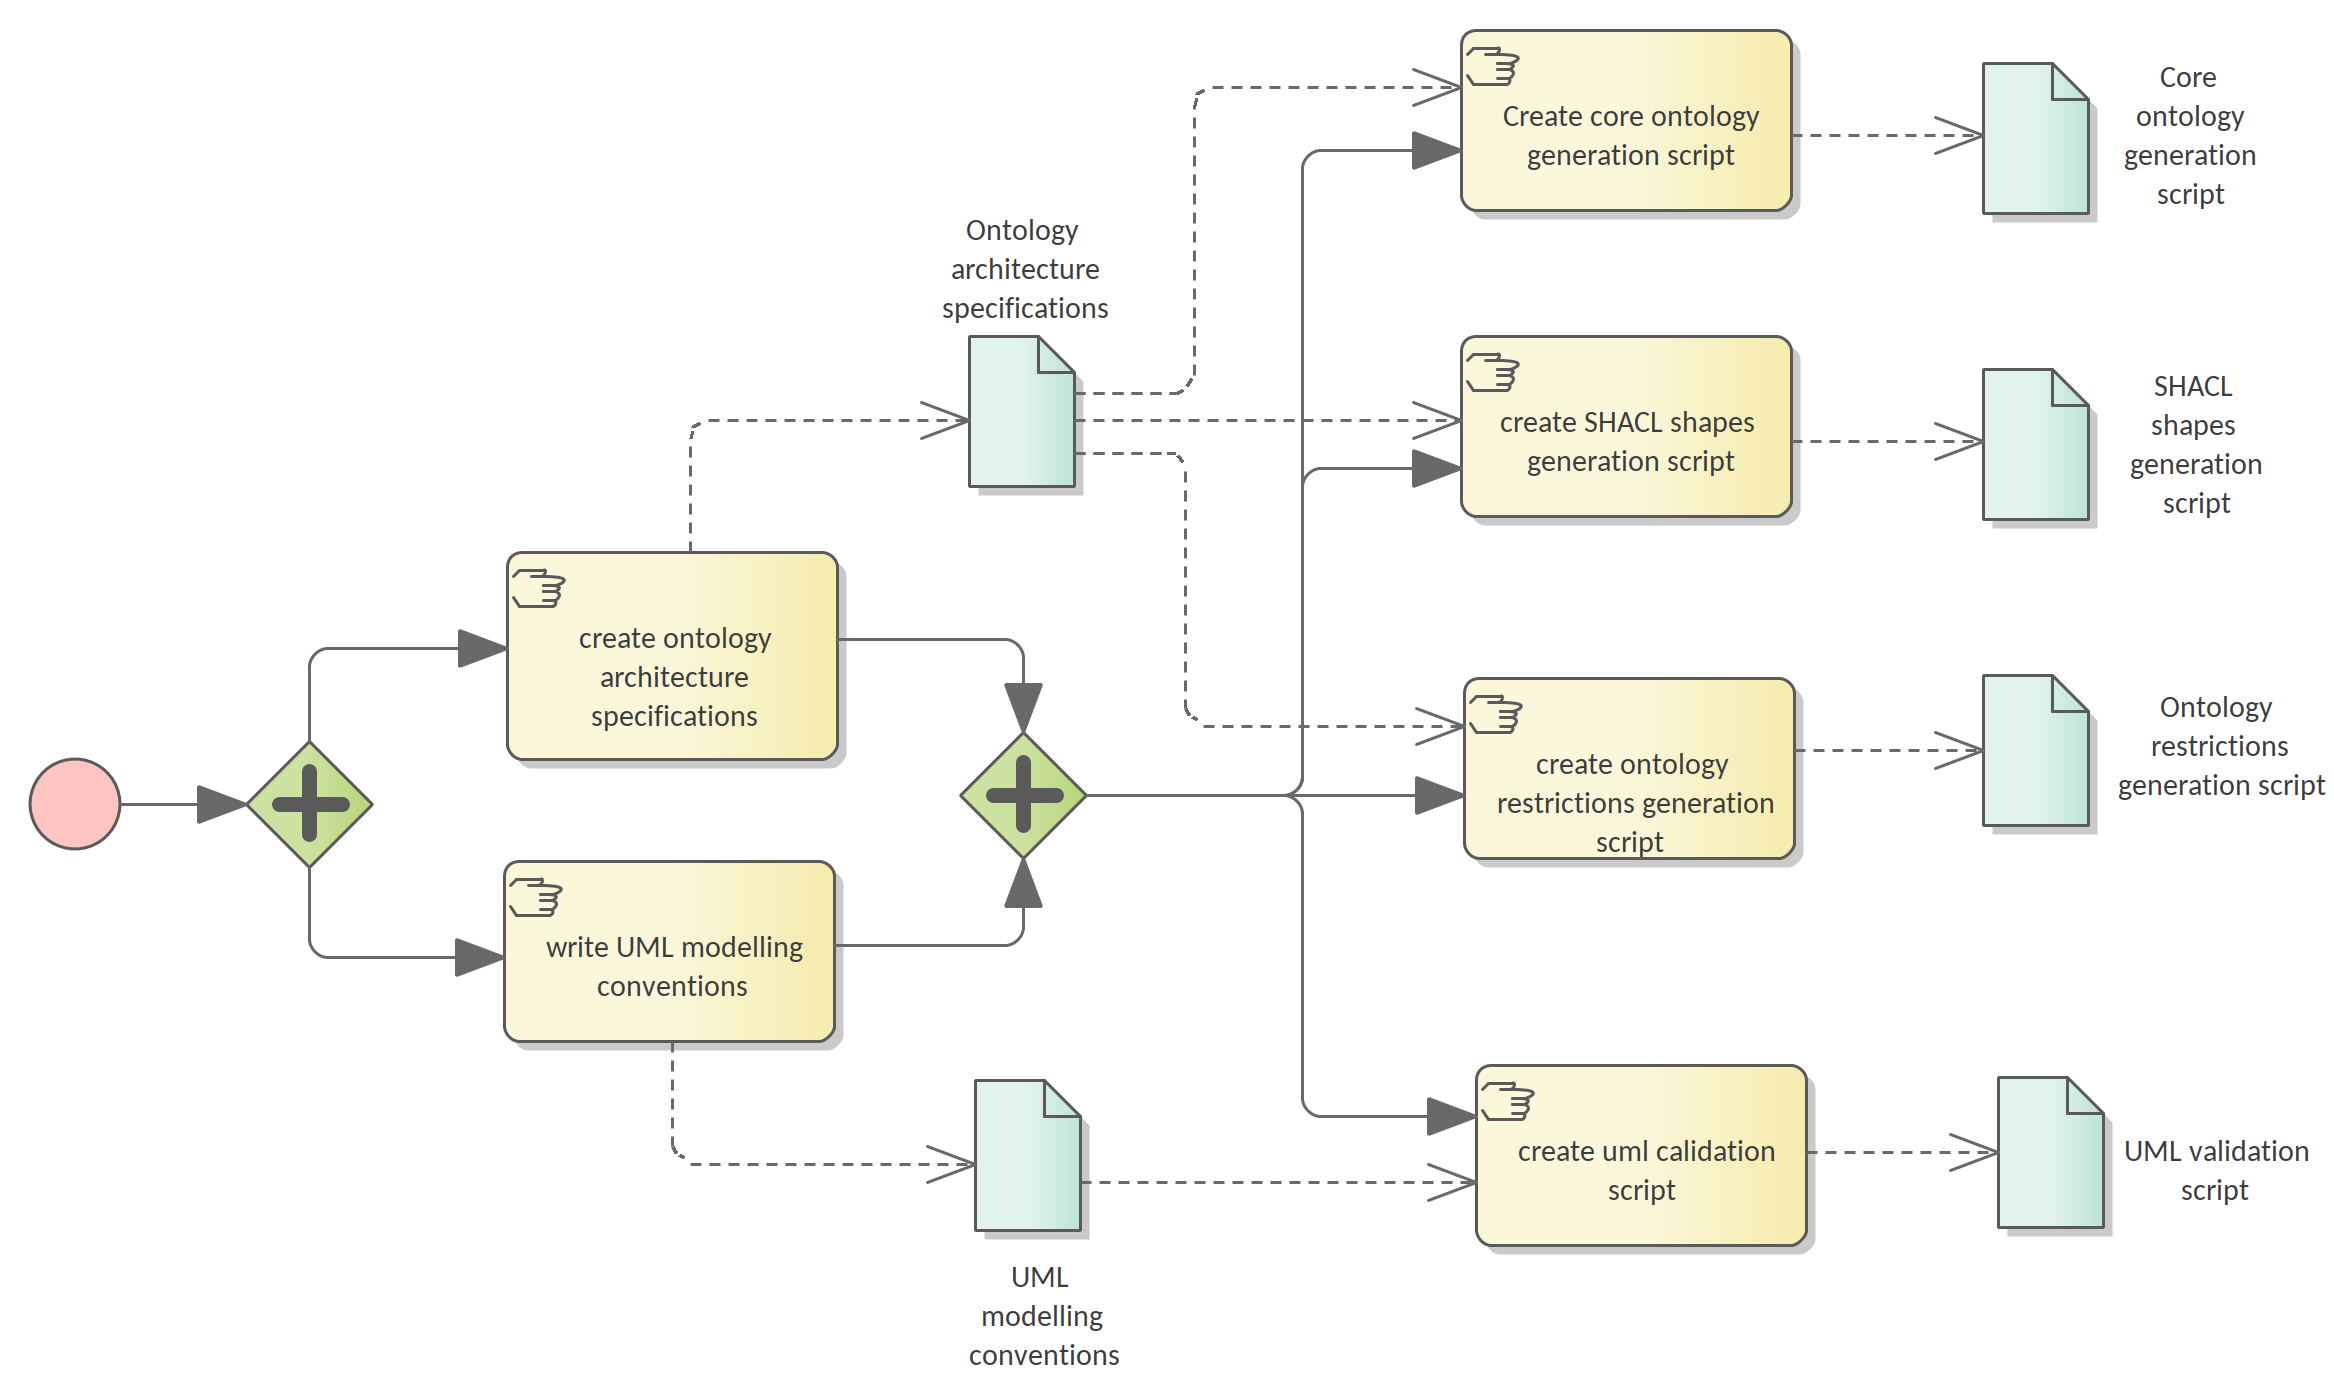
\includegraphics[width=\textwidth]{../img/uml2formalScriptCreation.png}
		\caption{Creation of the specifications documents and the UML transformation scripts}
		\label{fig:uml-transformation}
	\end{figure}
	
	The conceptual model must comply with a set of UML modelling conventions making it suitable input for the transformation scripts, which implement the same conventions. The two parallel actions starting the process are depicted in Figure \ref{fig:uml-transformation}.
		
	The UML conventions document serves, at large, as the requirements specification for the XSLT script that checks whether the UML conceptual model conforms to the conventions.
	
	The ontology architecture specification (this document) serves, at large, as requirement specifications for the development of three XSLT scripts to generate the formal ontology. These scripts can be developed independent of each other as they refer to different aspects of the formal ontology as described in Section \ref{sec:separation-conceprns}.
	
	The input for these scripts is the UML conceptual model, authored using Enterprise Architect, and serialised in XMI 2.5.1 format \cite{xmi2.5.1}.
	
	\subsection{Conceptual model revision}
	\label{sec:revision-cm}
	
	The current project runs under the assumption that the conceptual model is organised and expressed in accordance to the UML conventions specified in \citep{costetchi2020b}. However the conceptual model was developed well before the UML conventions were established. Therefore the model needs adjustments to conform to the conventions.  
	
	Having this assumption violated is a risk with critical impact. Therefore, an auxiliary process was developed (see Figure \ref{fig:revision-cm}) to continuously improve and correct the model in case it is non-conformant. 
	
	\begin{figure}[!ht]	
		\centering
		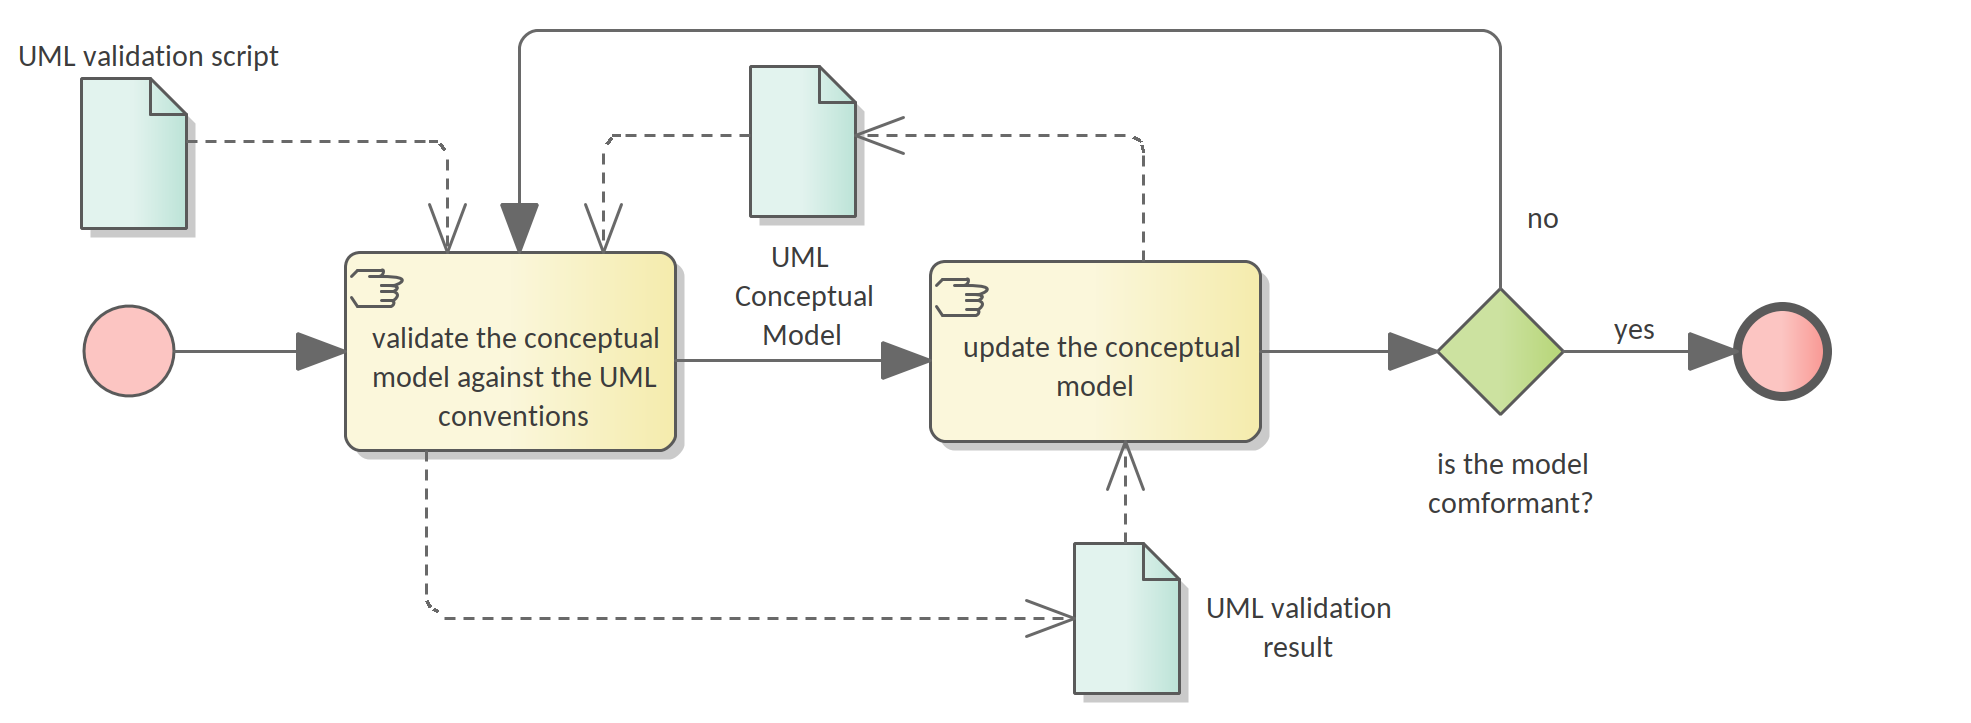
\includegraphics[width=.85\textwidth]{../img/conceptualModelRevision.png}
		\caption{Adjustment of the UML conceptual model guided by the validation script}
		\label{fig:revision-cm}
	\end{figure}

	The conceptual model revision is an iterative process. A validation script is developed in a preceding step (see Section \ref{sec:uml-transformation}). This script it is executed on the current conceptual model outputting a report. This report is comprised of errors and warnings with detailed description of what is the deviation from the UML conventions. It also provides hints for the conceptual model designer what are the necessary actions to resolve the issues.
	
	\subsection{Formal ontology generation}
	\label{sec:ontology-generation}
	
	The UML conceptual model constitutes the sole main input for three transformations scripts. Therefore, it is very important to ensure that the conceptual model is conform to the set of UML conventions \cite{costetchi2020b}. They ensure that the conceptual model represents an adequate input for the transformations script as they are developed based on the same set of conventions and assumptions.
		
	\begin{figure}[!ht]		
		\centering
		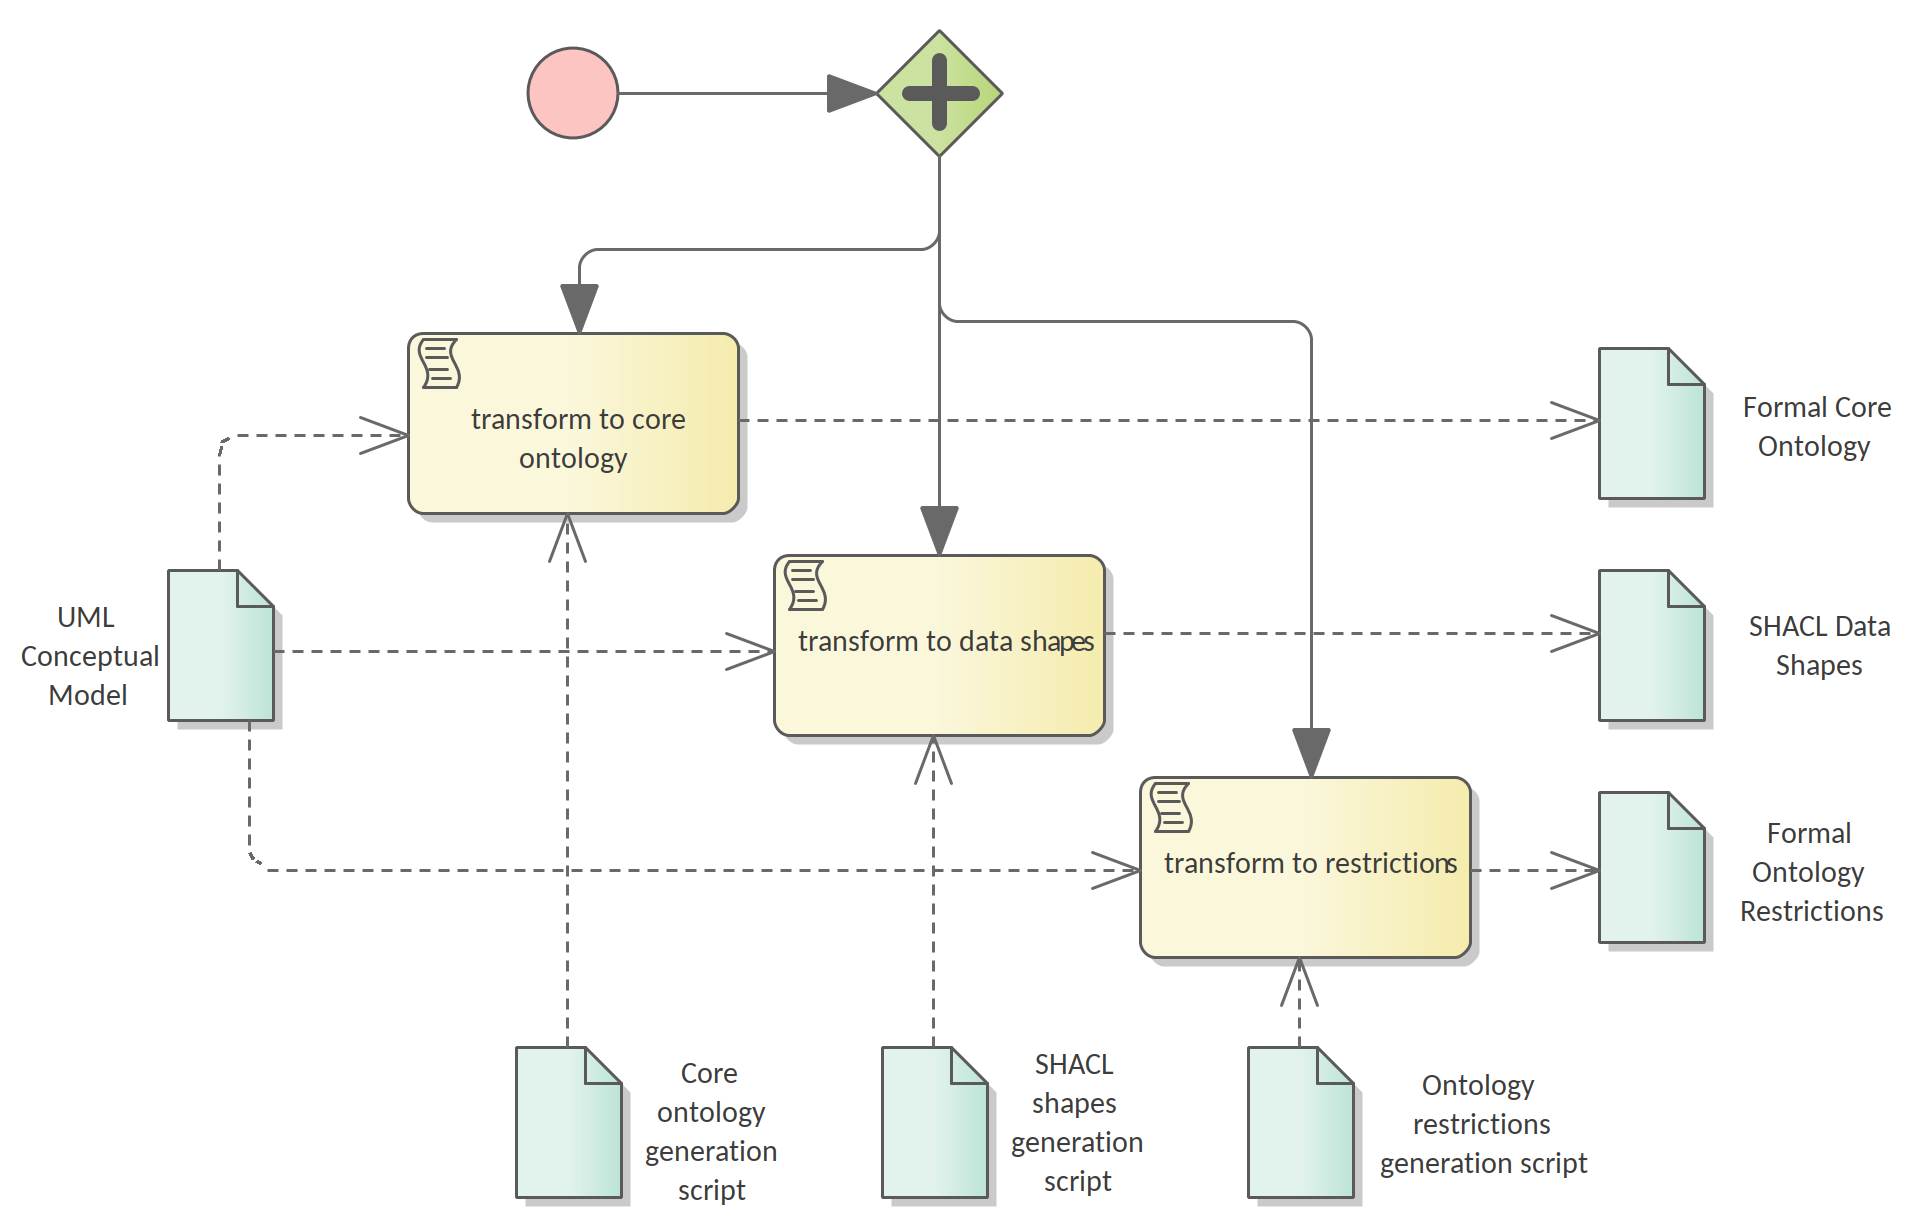
\includegraphics[width=0.8\textwidth]{../img/formalOntologyGeneration.png}
		\caption{Generation of the formal ontology from the UML conceptual model}
		\label{fig:ontology-generation}
	\end{figure}
	
	The transformation scripts, developed in a preceding step described in Section \ref{sec:uml-transformation}, are: the core ontology transformations script, the SHACL shapes transformation script, and the ontology restrictions generation script. Each are executed on the current conceptual model resulting in three output artefacts,  or three sets of outputs artefacts, that depends on the implementation decisions. Each output corresponds to one of the components of the eProcurement ontology addressed in Section \ref{sec:layers-components}: the formal core ontology, the SHACL data shapes, and the formal ontology restrictions. And this concludes the ontology generation process depicted in Figure \ref{fig:ontology-generation}. 	

	\subsection{XML to RDF data transformation}
	\label{sec:xml2rdf}

	In the introduction of this document, Section \ref{sec:context} explains that it is necessary to transform the current eProcurement data from XML formal (structured according to the standard forms) into RDF format. This process is depicted in Figure \ref{fig:transformation-proc}.
	
	The data must represent instances of the ontology generated in previous step explained in Section \ref{sec:ontology-generation}, which is structured according to the forthcoming eForms. This means that the transformations script must consider a carefully established conceptual mapping between the two standards in addition to implementing the format transformation itself. Figure \ref{fig:sub1} reflects that, and in addition, the XSD schemas, to which existent XML data conform, must be consulted and considered in the design and implementation process. 
	
	Current specification is agnostic to the technology used for implementing data transformation process. A noteworthy candidate is XSLT -- a language for expressing XML transformations. Yet, for the standard programming languages, such as Java, Python, JavaScript and many others, mature libraries to process XML and RDF are available.
	
	\begin{figure}[!ht]
		\centering
		\begin{subfigure}[b]{.48\textwidth}
			\centering
			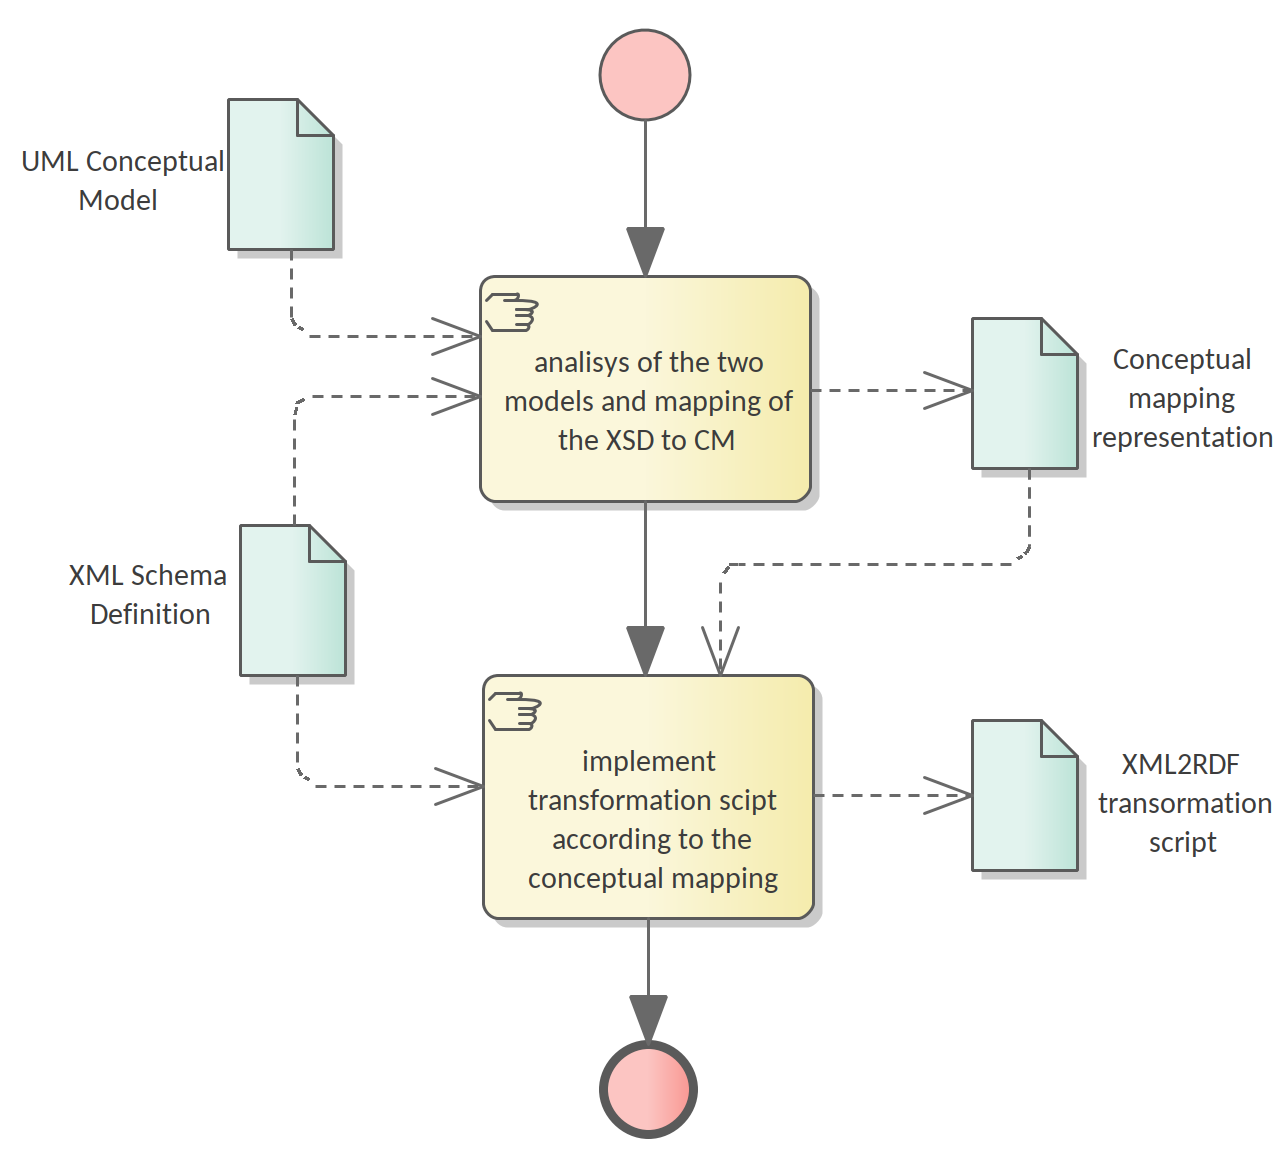
\includegraphics[width=1.05\linewidth]{../img/xml2rdfScriptCreation.png}
			\caption{Implementation of the XML transformations script based on the mappings from XSD schemas onto the conceptual model}
			\label{fig:sub1}
		\end{subfigure}%
		\quad
		\begin{subfigure}[b]{.48\textwidth}
			\centering
			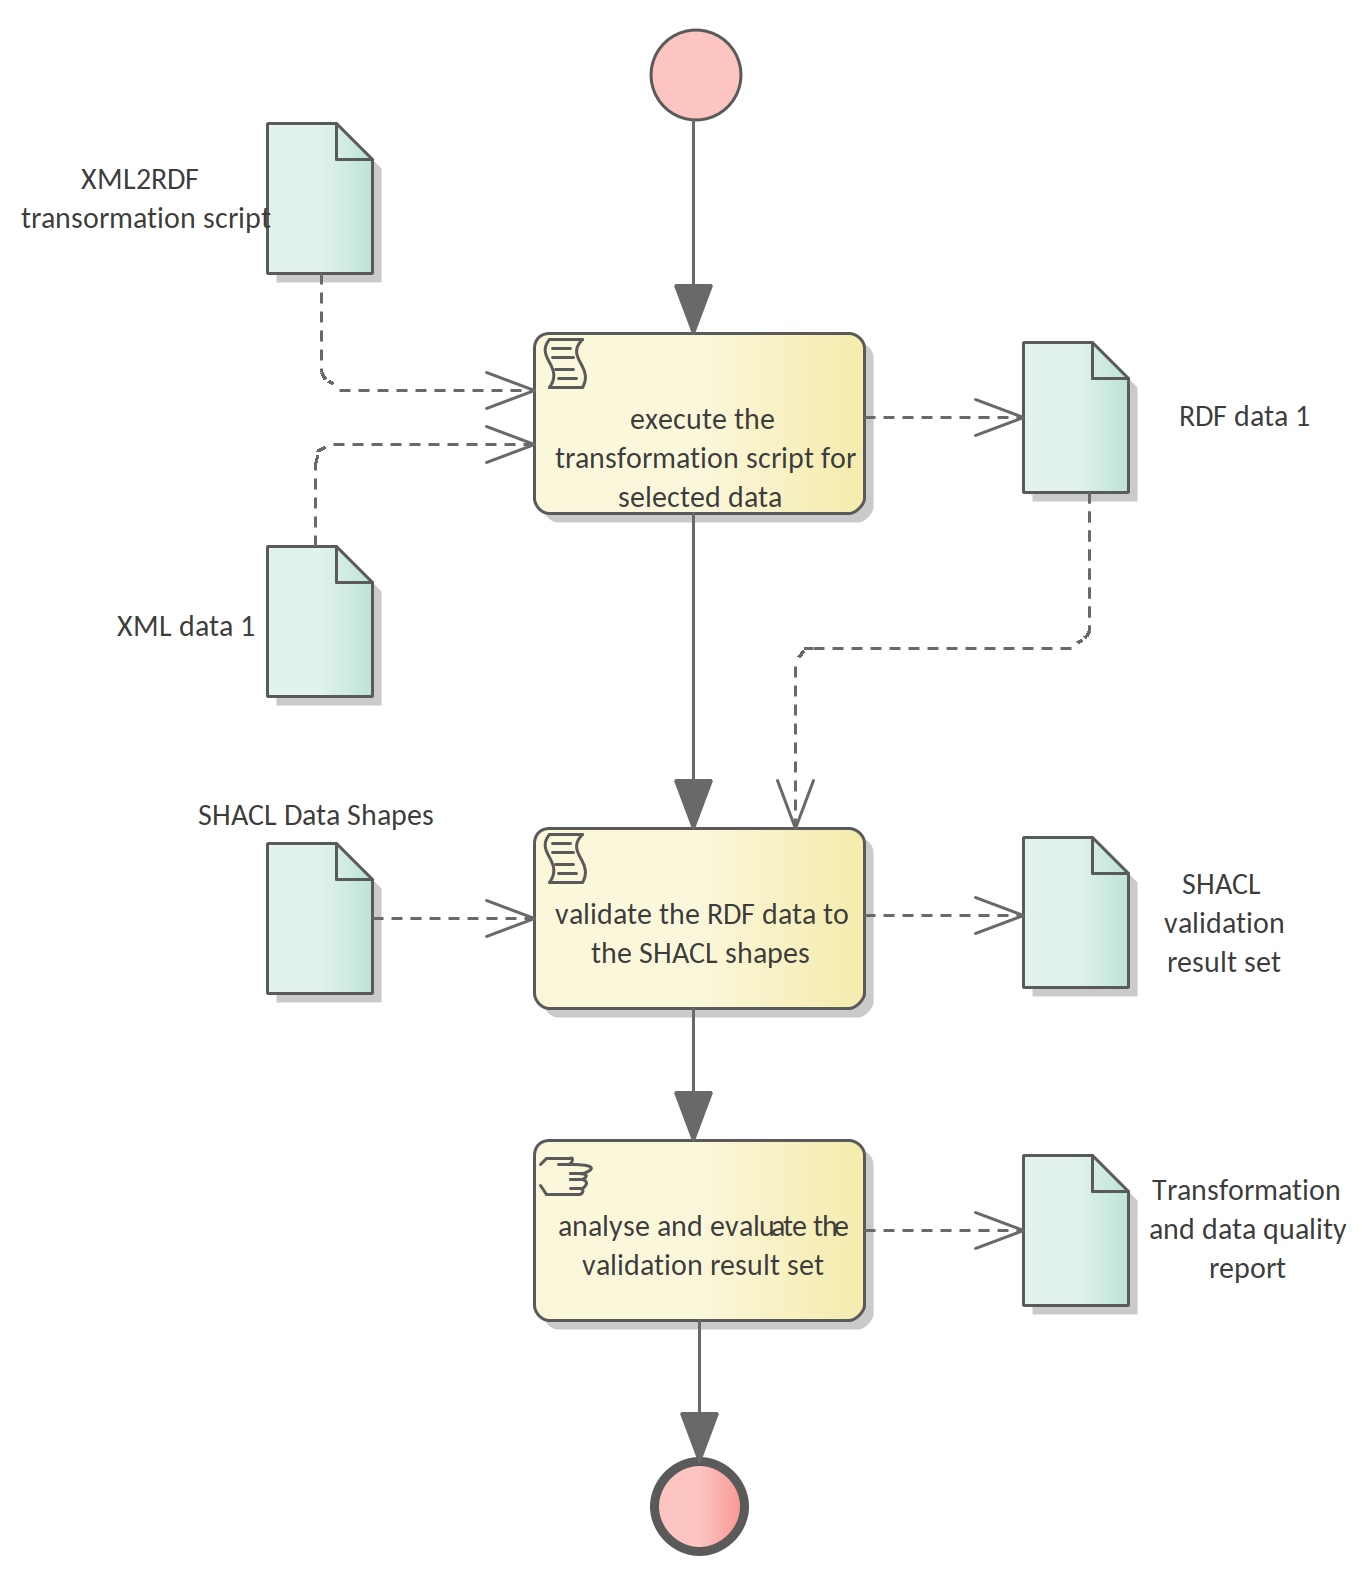
\includegraphics[width=1.05\linewidth]{../img/xmlDataTransformation.png}
			\caption{Transformation of the existent eProcurement XML data into RDF representation and validating the end result conformance}
			\label{fig:sub2}
		\end{subfigure}
		\caption{XML to RDF data transformation}
		\label{fig:transformation-proc}
	\end{figure}

%	The process is divided into two subprocesses: first the XML transformations script is developed, depicted in Figure \ref{fig:sub1}; second the transformation process is executed resulting in the RDF data, depicted in Figure \ref{fig:sub2}.

	The execution of data transformation process (see Figure \ref{fig:sub2}) unfolds in three steps as follows. First, the selected data is fed as input to the transformation script. The output RDF data are then validated for conformance to the formal ontology using the SHACL data shapes. The validation output is a report in RDF format listing possible violations of the data. This report is transformed into a human readable form using a SPARQL query and used to interpret the conformance of the data, and eventually spot mistakes in the transformation script of in the data shapes.   
	
	These reports must be used during the transformation script development, as additional stress tests for whether the script performs correctly or it needs further adjustments. Of course, these reports may indicate problems stemming from either the transformation script, the input data or the SHACL shapes. Therefore, a developer's assessment is necessary to decide on the source of the issue and provide the necessary feedback. The script development process may be considered complete, when for a random set of input data, the analysts and developers can assert that only the input data caused the exceptions. The data driven conformance exceptions constitute an important input in the ontology validation step of the process presented in Section \ref{sec:ontology-validation}.
	
	\subsection{Ontology evaluation}
	\label{sec:ontology-validation}
	
	The ontology evaluation process aims at assessing how well the use cases listed in the functional requirements (see Section \ref{sec:functional-requirements}) are enabled and supported by the formal ontology and consequently the conceptual model. The evaluation process needs to be designed elsewhere, but at this stage it is possible to foresee two processes that needs to take place: loading the data into a triple-store and querying the data and analysing the result-set for fitness. 

	\begin{figure}[!ht]		
		\centering
		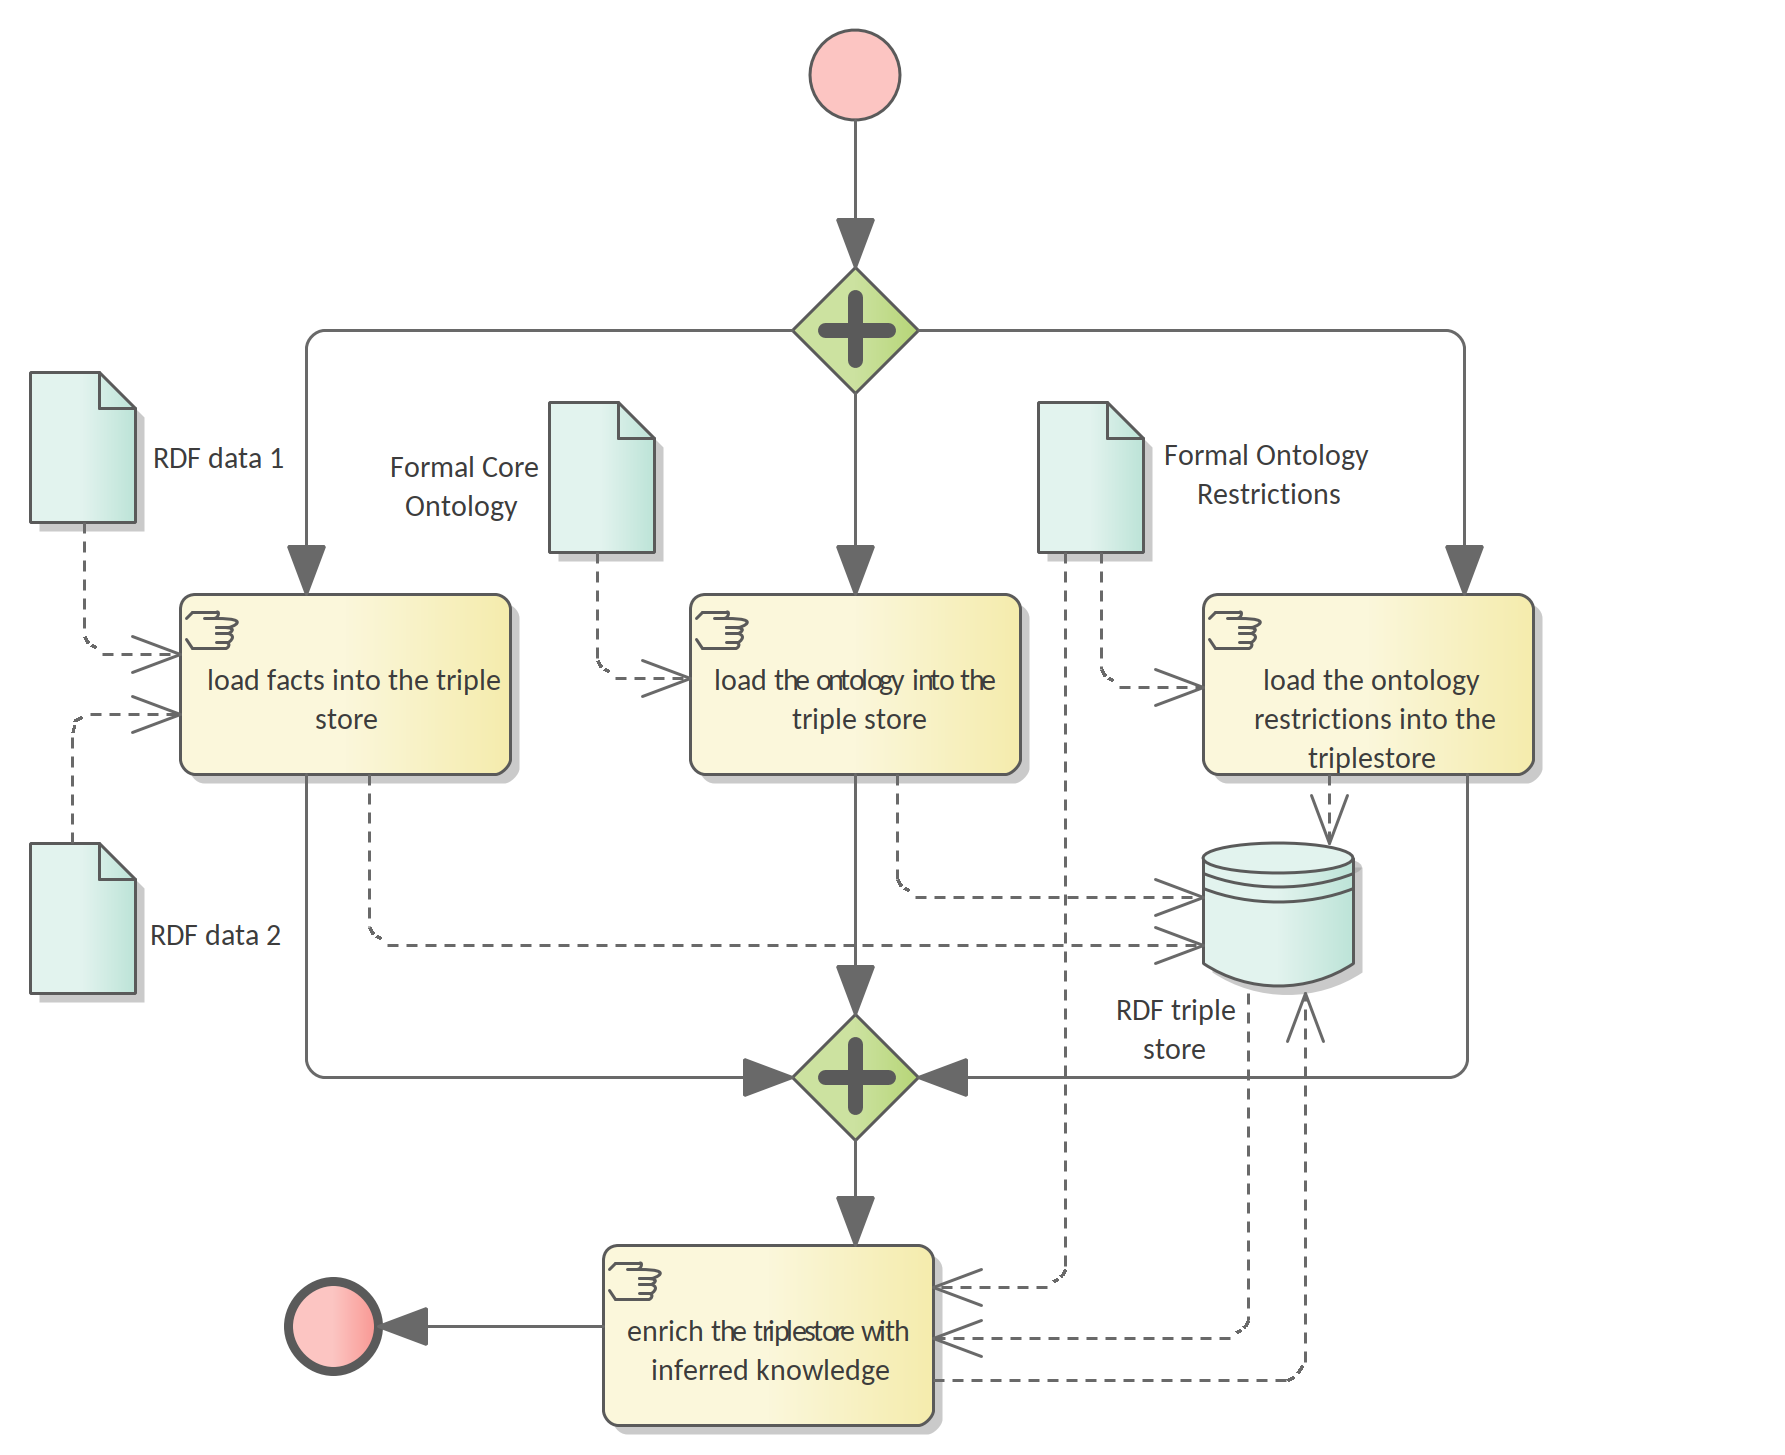
\includegraphics[width=0.86\textwidth]{../img/loading-data.png}
		\caption{Loading the data into the triple store}
		\label{fig:loading-date}
	\end{figure}

	Figure \ref{fig:loading-date} depicts the process of loading data into a triple store. Three components must be ingested before it is ready for query: (a) the RDF datasets generated from the existent XML datasets, (b) the core ontology and (c) the formal ontology restrictions. These three components correspond to a complete ontology where the model and the data, i.e. ABox and TBox (see Section \ref{sec:model-data}), are brought together into a whole.
	
	The triple-store organisation, whether it acts as an eProcurement data dissemination service, URI dereferencing or other publications related issues is not in scope of the current architecture specification. Nevertheless, the data organisation and dissemination should be treated elsewhere in detail considering the best practices for publishing linked data \cite{bizer2009emerging}.
	
	For the purposes of the evaluation efforts, the TBox axioms, i.e. the core ontology and the formal restrictions, must be saved in a dedicated graph.  It is recommended that the instance data is also partitioned into a set of logical and manageable graphs.  

	Once the data and the ontology are loaded, the benefits of the underlying logical formalism can be drawn: checking the consistency of the data dn model and inferring new knowledge from the existent one. In case the triple store has an incorporated reasoner it should be enabled following an OWL 2 direct semantics described in Section \ref{sec:semantics}. Otherwise an external reasoner such as Fact++ \cite{tsarkov2006fact++}, Pellet \cite{sirin2007pellet}, HermiT \cite{shearer2008hermit} or CB \cite{kazakov2009consequence}, must be used to enrich the triple-store. A comparison of OWL 2 EL reasoners is provided in \citep{dentler2011comparison}. It is, however, dated and a thorough state of the art research needs to be considered before commencing the work on reasoning. 
	
	It is not yet possible to decide at this stage about the range of reasoning capabilities that can be engaged for the eProcurement ontology. Experiments must be conducted on available data to evaluate the speed of reasoning against the expressivity of the considered formalism expressivity and the coverage of inference rules as described in Section \ref{sec:expressivity}.
	
	In principle, it is possible to engage with ontology evaluation process directly after the data loading steps and skipping the inferencing step, but the range of potential answers will be limited to an extent, which currently is not possible to evaluate.
		
	\begin{figure}[!ht]		
		\centering
		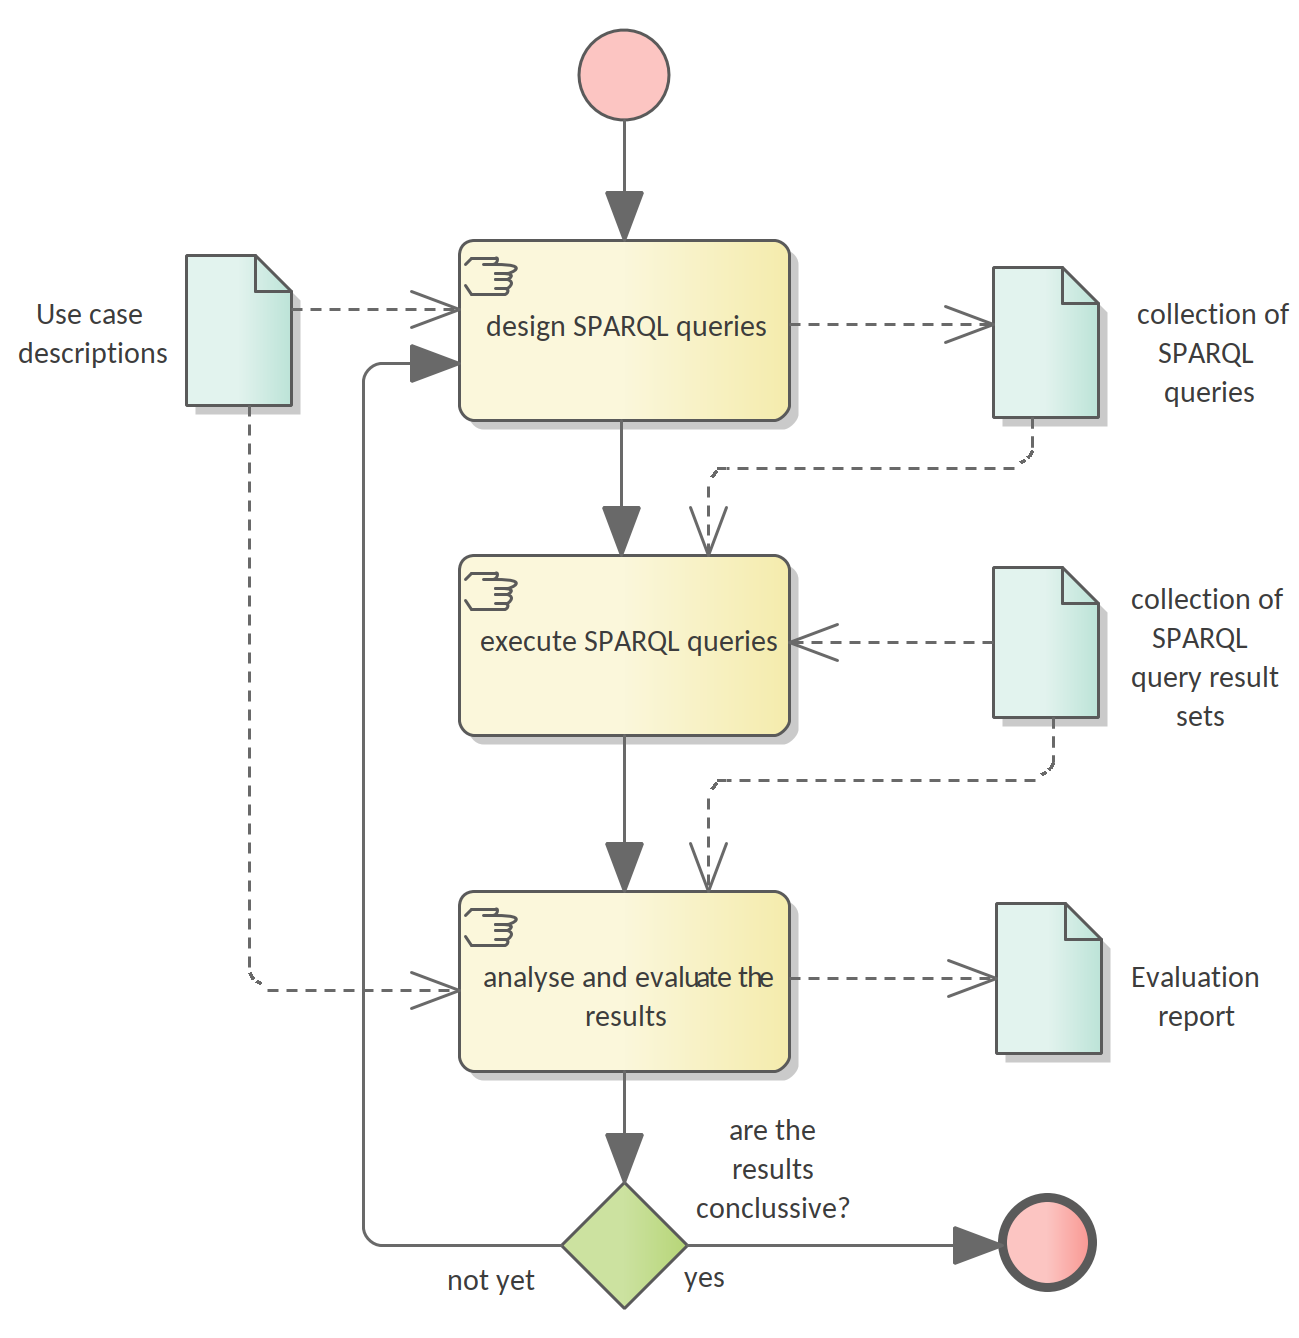
\includegraphics[width=0.6\textwidth]{../img/conceptualValidation.png}
		\caption{Conceptual validation of the eProcurement ontology against selected use cases}
		\label{fig:ontology-validation}
	\end{figure}
	
	Once the triple store is enriched with inferred information, it can be used to address the use case related information needs. The process is depicted in Figure \ref{fig:ontology-validation}. 
	
	Each use case carries a set of information needs which must be derived and expressed in the form of SPARQL queries. The ontology evaluation process commences with developing a collection of such queries. Then they are executed on the triple-store and the result sets are collected. Empty sets are also important results as they indicate possibly an ill-formed query, a lacuna in the existent data or an incorrectly modelled ontological segment.
	
	The result sets are evaluated and aggregated into a conclusive report explaining the strong and weak points of developed ontology in addressing the selected use cases given the existent data.  
	
	
	
	
	